\section{Introducción}
	

El propósito de este capítulo es actualizar los coeficientes del indice CAPECO creado por el INDEC para utilizar en el marco del Censo 2001. Para ello utilizaremos los datos de la EPH correspondientes al tercer trimestre de 2010 de modo que coincida con el momento de relevamiento de datos del Censo 2010 (27 de octubre de 2010). Dado que nos concentramos en el Aglomerado Gran Buenos Aires, solamente tomaremos los datos pertenecientes a los aglomerados de Ciudad de Buenos Aires y Partidos del Gran Buenos Aires.  

Basándose en el paradigma del capital humano  \cite{mincer,beckar,schultz1961,schultz1962}, el modelo toma un conjunto de variables que puedan servir a aproximar el ingreso que perciben. Fundamentalmente, se considera el salario como una función de la productividad y la misma depende de factores como la experiencia y los años de escolaridad. Otras variables inciden en el mismo, pero no son relevadas en el Censo por lo cual quedan al margen del análisis. Al mismo tiempo, el género es un elemento a considerar dadas las iniquidades salariales empíricamente verificadas en diversos mercados laborales en el mundo y en la Argentina. 

Por lo tanto, se utilizan estos supuestos para construir un modelo que intente aproximarse al ingreso. Como se estableció previamente, el CAPECO intenta aproximar el Ingreso Per Cápita Familiar (IPCF). Sin embargo, al partir del modelo del capital humano se hace foco en los ingresos laborales. Si bien existen otras fuentes, éste continúa siendo el ingreso primordial de los hogares. A su vez los supuestos del capital humano para dar cuenta de los determinantes de este ingreso hace que el modelo resulte más preciso y legible. Incluir el ingreso total de las personas incluiría mayor fuente de variación que no sería explicada por el modelo. 

Por lo tanto, el modelo subyacente al CAPECO utiliza las siguientes variables para aproximarse al ingreso individual de las personas, previa transformación logarítmica de éste para establecer una relación \textit{log-lineal}, y utilizando al varón adulto de 35 años o más sin años de escolaridad como caso base o registro:

\begin{itemize}
	\item  Años de escolaridad primaria (\textit{aeprim})
	\item Años de escolaridad secundaria (\textit{aesec})
	\item Años de escolaridad universitaria (\textit{aeuniv})
	\item Varón entre 14 y 24 años (\textit{v14to24})
	\item Varón entre 25 y 34 años (\textit{v25to34})
	\item Mujer entre 14 y 24 años (\textit{m14to24})
	\item Mujer entre 25 y 34 años (\textit{m25to34})
	\item Mujer entre de 35 años o más (\textit{m35mas})
\end{itemize}

De esta manera el modelo queda especificado del siguiente modo:

$$Ln Y_n = Ln Y_0 + \beta_0 aeprim + \beta_1 aesec + \beta_2 aeuniv + $$
$$\beta_3 v14to24 + \beta_4 v25to34 +  \beta_5 m14to24 +  $$
$$\beta_6 m25to34 +  \beta_7 m35mas +  \cdots + \epsilon $$


El modelo original en base a datos de 2001 incluye la región a la que pertenece la persona (los ingresos varían según la región del país) y si la persona percibía jubilación o pensión. Sin embargo en este trabajo únicamente analizamos el modelo para la región del Aglomerado Gran Buenos Aires y en el censo 2010 no se preguntó en el formulario básico sobre la percepción de jubilación o pensión.

Este capítulo sigue la siguiente estructura. En primer lugar se pasa a hacer un análisis descriptivo de las variables utilizadas en el modelo. En segundo lugar, se implementa el modelo subyacente al CAPECO y se analizan sus resultados. En tercer lugar, se pasa a construir los coeficientes del índice CAPECO en base a la estimación de los parámetros del modelo. Finalmente se analiza la relación del CAPECO y el Ingreso Per Cápita Familiar.

\section{Exploración de las variables intervinientes}

En primer lugar analizamos la distribución del ingreso de la ocupación principal en escala logarítmica. 

\begin{figure}[!htb]
	\centering
	\textbf{Kernel density plot del Ingreso de la ocupación principal en escala logarítmica}\par\medskip
	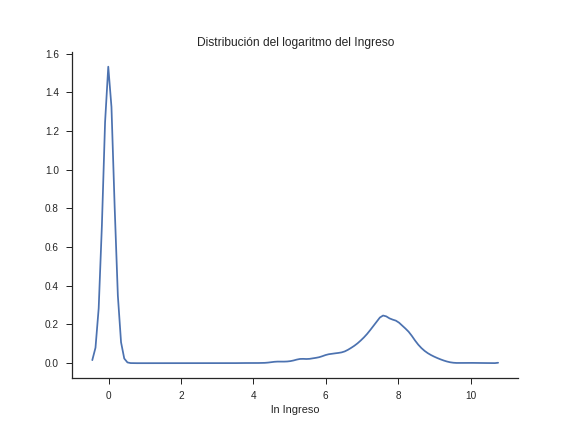
\includegraphics[scale = 0.5]{../img/capitulo3/kdePlotIngreso1.png}
	\caption{En la figura se puede observar cómo la distribución tiene dos picos: aquellos que no tienen ingresos y aquellos con ingresos.}
\end{figure}

Existe la mayoría de la población no percibe un ingreso profesional, lo cual es de esperar ya que su condición de actividad así lo indica (menores de 14 años, estudiantes, jubilados, desocupados, etc). 

\begin{figure}[!htb]
	\centering
	\textbf{Ingreso de la ocupación principal según condición de actividad}\par\medskip
	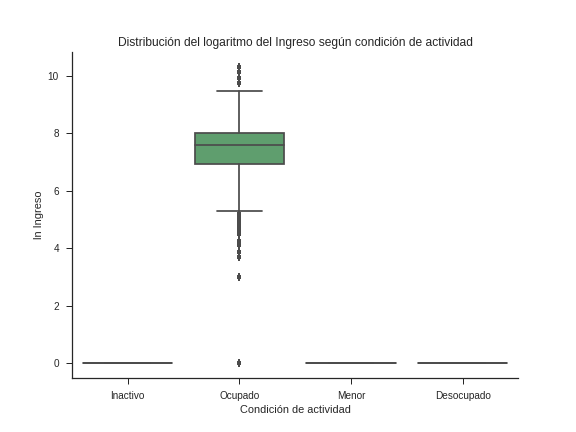
\includegraphics[scale = 0.5]{../img/capitulo3/kdePlotIngreso2.png}
	\caption{En la figura se puede observar la distribución para cada categoría de actividad. Como es de esperar, solo los ocupados registran ingresos de las ocupaciones principales.}
\end{figure}

En ese sentido, procedemos a analizar únicamente a la población que tiene ingresos y una ocupación. Esto implica una limitación a la hora de percibir el conjunto de los ingresos (de los cuales los laborales, si bien una parte importante, constituyen solo una porción). Como se puede ver en el gráfico la mayoría de los ingresos provienen tienen como fuente la ocupación principal (para el 75\% de los casos los ingresos de lo ocupación principal explican \textit{al menos} el 67.5\% del ingreso total). Al mismo tiempo, las personas con trabajo que no perciben ingresos y tienen trabajo constituyen un caso extremo que perjudica la performance del modelo. Puede deberse a que el trabajo es reciente y aún no cobraron el primer salario.

\begin{figure}[!htb]
	\centering
	\textbf{Proporción del ingreso salarial sobre el total según condición de actividad}\par\medskip
	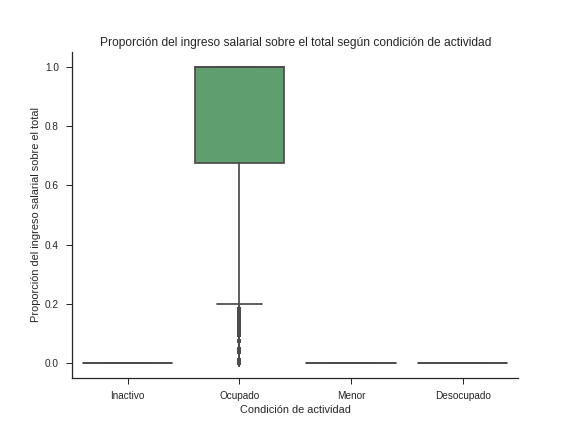
\includegraphics[scale = 0.5]{../img/capitulo3/ingresoSalarialVtotal.png}
	\caption{En la figura se puede observar que el grueso de los ingresos de los ocupados proviene de la ocupación principal.}
\end{figure}

En términos de género se observa un ingreso menor por parte de las mujeres. La media del ingreso de la mujer es el 93.84 \% de la del varón (en escala logarítmica) mientras que la mediana representa el 95.31 \% de la del varón. En términos de ingreso, dicha diferencia se amplía a 70.55\% para la media y 69.57\% para la mediana. 


\begin{figure}[!htb]
	\textbf{Ingreso de la ocupación principal según género}\par\medskip
	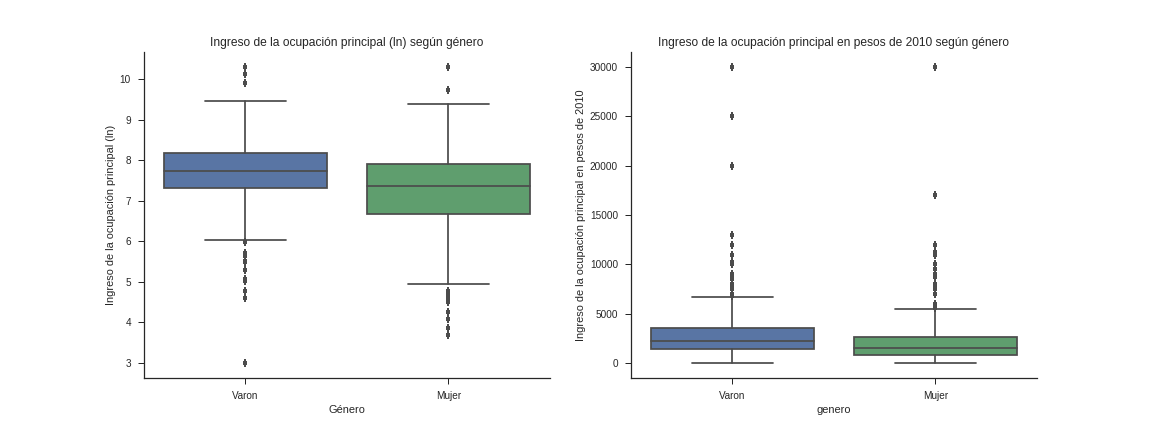
\includegraphics[scale = 0.4]{../img/capitulo3/ingresoVgenero.png}
	\caption{En la figura se puede observar que los varones tienen un ingreso superior en promedio al de las mujeres.}
\end{figure}

Es necesario a su vez dar cuenta de las relaciones existentes entre la edad y el ingreso como así también entre éste y los años de escolaridad. 

\begin{figure}[!htb]
	\textbf{Ingreso (ln) según género y escolaridad}\par\medskip
	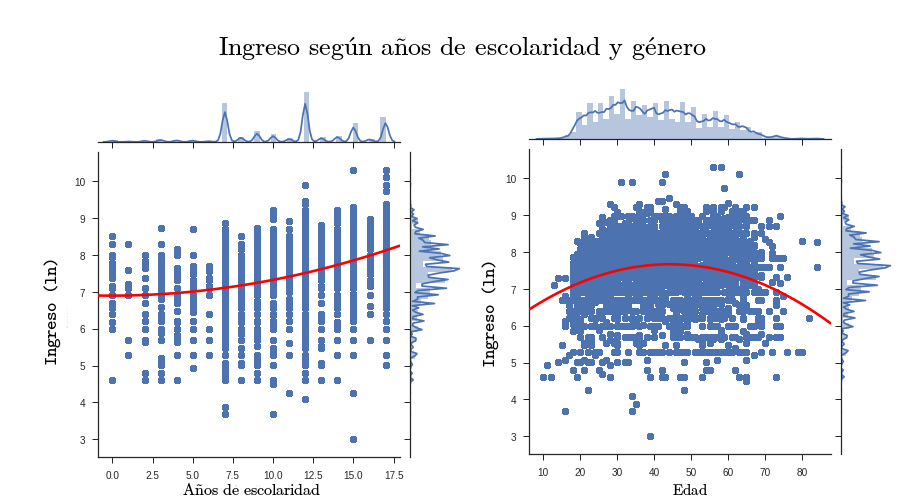
\includegraphics[scale = 0.4]{../img/capitulo3/ingresoVedadVescolaridad.png}
	\caption{.}
\end{figure}

Como se puede observar existe una relación no lineal entre estas variables. En lo que corresponde a la edad, parece haber una relación creciente hasta pasados los 30 años. Llegada esa edad hay un amesetamiento por el cual no hay incrementos salariales a partir de la edad, para luego comenzar un proceso descendente (el año que inicia el cambio de tendencia hacia el descenso cambia de acuerdo al género: en las mujeres este proceso parece ser durante los 50s mientras que en los hombres en los 60s, lo que coincide con las diferencias en las edades jubilatorias legales).

El comportamiento de la variable es similar (a pesar de una media de ingreso superior en los hombres). A mayor escolarización mayor salario. Pero esta relación no es lineal, sino que cada año de escolaridad de los tramos superiores ofrece mayores retornos que cada año de los tramos inferiores de escolaridad. Así por ejemplo un año adicional de universidad incrementa más el salario que un año adicional de primaria.

 \begin{figure}[!htb]
 	\textbf{Ingreso (ln) según género y escolaridad - Mujeres}\par\medskip
 	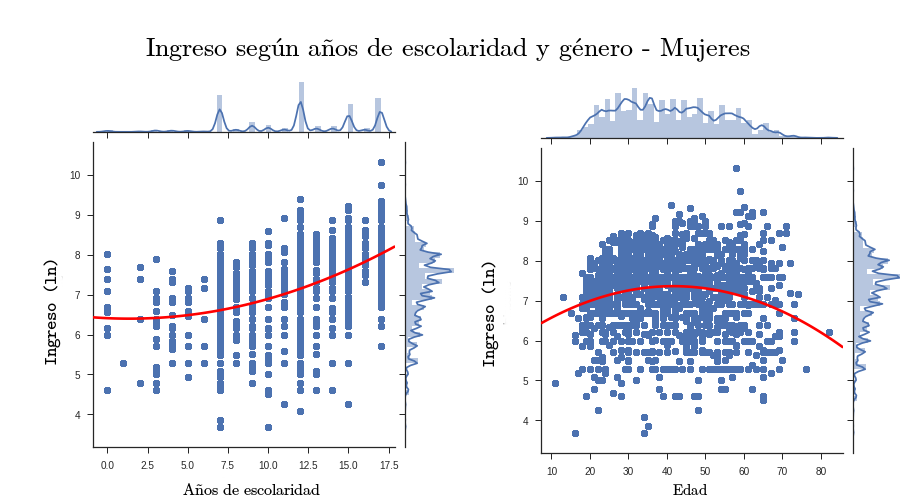
\includegraphics[scale = 0.4]{../img/capitulo3/ingresoVedadVescolaridadMujeres.png}
 	\caption{.}
 \end{figure}

 \begin{figure}[!htb]
 	\textbf{Ingreso (ln) según género y escolaridad - Varones}\par\medskip
 	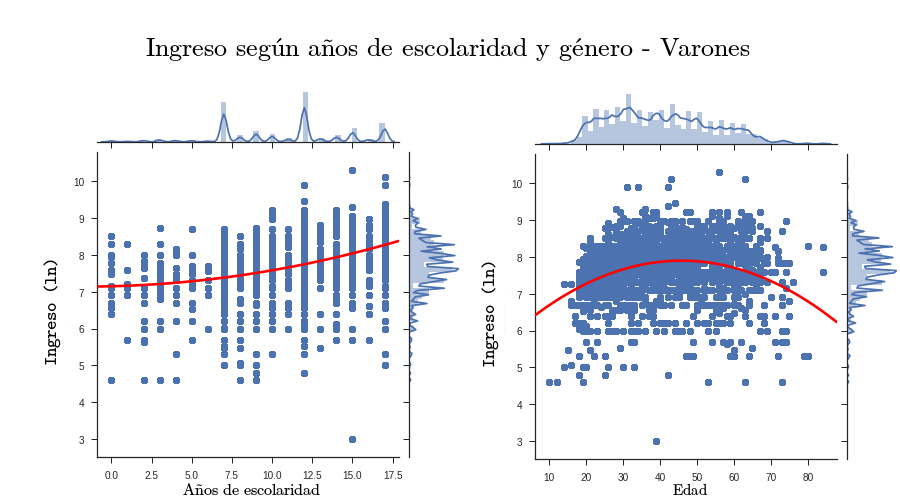
\includegraphics[scale = 0.4]{../img/capitulo3/ingresoVedadVescolaridadVarones.png}
 	\caption{.}
 \end{figure}
 
 Finalmente podemos ver la matriz de correlación. La mujer leve correlacionpositiva con escolaridad (0.125839).  negativa con inrgeso (-0.267508) y ninguna con edad. Escolaridad postivai con ingreso 0.401385, levemente ocn la edad -0.112473. casi inexistente entre edad e ingreso, 0.046077 porque la relacion es una curva. 
 
  \begin{figure}[!htb]
  	\centering
  	\textbf{Matriz de correlación - Variables seleccionadas}\par\medskip
  	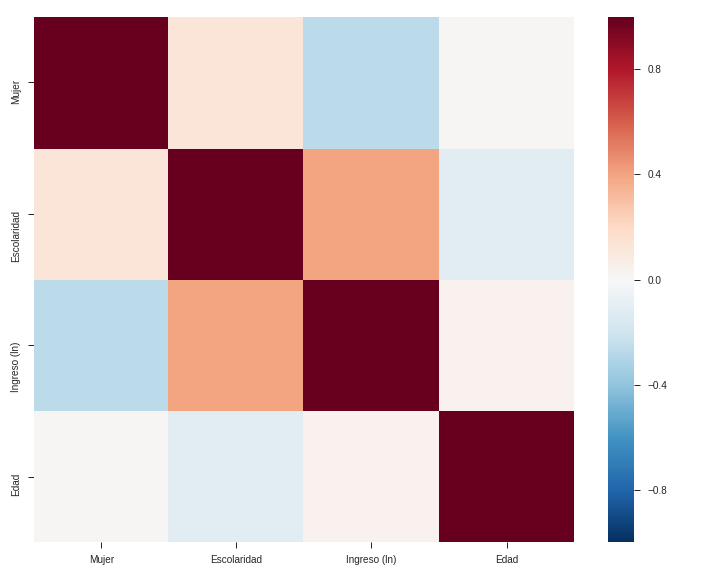
\includegraphics[scale = 0.4]{../img/capitulo3/corrMatrix.png}
  	\caption{.}
  \end{figure}
  
  Podemos ver que hay una leve tendencia a que, dentro de las personas con un trabajo, las más jóvenes tengan más años de escolaridad que las mayores. Esto puede ser así porque el nuevo mundo del trabajo demanda mas cali.
  
    \begin{figure}[!htb]
    	\centering
    	\textbf{Años de escolaridad según edad}\par\medskip
    	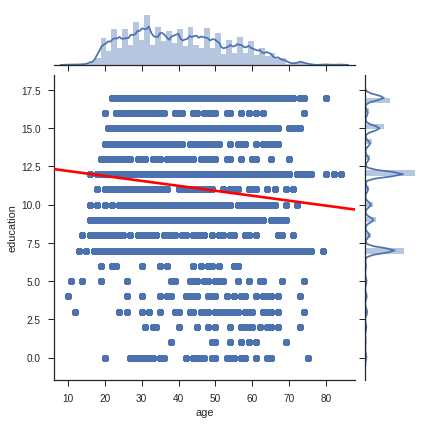
\includegraphics[scale = 0.4]{../img/capitulo3/educVage.png}
    	\caption{.}
    \end{figure}
 
\section{El modelo y sus resultados}
A continuación procedemos a correr el modelo para todos los individuos con ingresos y que se encuentren empleados. La performance del mismo es disimil. Si bien por un lado todos los parametros son estadisticamente significativos para cualquier nivel de confianza, el modelo en su ocnjunto alcanza un R2 de solo 27\%. Esto quiere decir que este modelo solo puede dar cuenta del 27\% de la variabilidad del logaritmo del ingreso. De todos modos es importante recordar que este modelo no considera elementos fundamentales para el ingreso como la cantidad de horas trabajadas o la rama en la que se desempeña cada persona. Diferentes ramas tienen diferentes productividades y por lo tanto pagan diferentes salarios.

De todos modos, el objetivo último de este modelo es ofrecer fundamento para los coeficientes del CAPECO. En todo caso veremos al final que capacidad tiene el CAPECO para dar cuenta de la variabilidad del ingreso.

En primer lugar, el intercepto da cuenta del ingreso esperado para un hombre adulto de 35 años o más con 0 años de escolaridad en cualquiera de los 3 niveles. Este constituye el caso base o registro con el cual compararemos al resto de los casos.

En segundo lugar los coeficientes dan cuenta de una relación Log-Nivel, esto quiere decir, por tomar el ejemplo del primer coeficiente (años de escolaridad primaria), que un año de escolaridad primaria ofrece un incremento de 7.87\% en el ingreso. Dicho de otro modo, un hombre adulto de 35 años o más con 1 año de escolaridad, gana un 7.87\% más que nuestro caso base (un hombre adulto de 35 años o más con 0 años de escolaridad). Del mismo modo, un año de escolaridad secundaria ofrece un incremento de 8.38\% y un año de escolaridad superior ofrece 12.21\%. Como es de esperar, los rendimientos no son lineales. Esto quiere decir que en el mercado laboral se valorizan más los años de escolaridad secundaria que los de primaria y los de educación superior a los de secundaria. El supuetso subyacente es que la productividad del trabajo aumenta con la capacitación que ofrece el sistema educativo.

En tercer lugar, los parámetros vinculados a la edad para los hombres, actúan como penalidades. Es decir, se supone que la edad conlleva experiencia y con ella mayor productividad. A su vez, el ciclo vital conlleva que los gastos de personas de tramos etarios superiores sean mayores. Es por ello que los hombres entre 14 y 24 años de edad sin años de escolaridad, ganarán un 42.12\% menos que el caso base, manteniendo todas las otras variables consideradas en el modelo constantes. A su vez, un hombre entre 25 y 34 años sin años de escolaridad tendrá un ingreso 15.47\% menor al del caso registro.

Finalmente, es necesario tomar en consideración el efecto del género conjugado con la edad. En primer lugar, parámetro que da cuenta del efecto del género al comparar una mujer de 35 años o más sin años de escolaridad con nuestro caso base (un hombre de idénticas características), nos dice que dicha mujer tendría un ingreso 58.43\% menor. Para los otros tramos de edades, una mujer entre 14 y 24 años dicha diferencia es de un 92.96\% menos y entre 25 y 34 años es de 62.64\% menos. 



\section{Construcción del CAPECO y sus coeficientes}

VEMOS COMO LAS MUJERES NECESITAN MAS EDUCACION PARA COMPENSAR Y DE L AMISMA MANERA LOS MAS JOVENES TIENEN MAS EDUCACION POR ESO SE ACHICO LA BRECHA CON RESPECTO A 2001

\section{El CAPECO como predictor del Ingreso Per Capita Familiar}